\section{Quantum Capacity of Quantum Channels}

\subsection{Coherent Information and Quantum Capacity}

We now concern ourselves with the transmission of quantum states. Recall that both classical and private communication models concerned themselves with reliable transmission of classical bits. This was typically modelled with orthogonal basis states. However, transmission of arbitrary quantum states involve dealing with more complex phenomenon such as entanglement.

Suppose Alice prepares a pure state $\phi_{AA'}$ and inputs the system $A'$ to a quantum channel $\mathcal{N}_{A' \rightarrow B}$. This transmission gives us the bipartite state $\rho_{AB} = \mathcal{N}_{A' \rightarrow B} (\phi_{AA'})$. An intuitive way of measuring the information throughput is to measure how uncertain the receiver is of the input given the received quantum states. This aligns with the definiton of conditional entropy. Since we concerned with reducing the conditional entropy, we can define an analogous measure that we seek to maximize instead.

\begin{definition}[Coherent Information of a Quantum State]
The coherent information of a state that arises from the channel is defined as:
$$I(A \rangle B)_{\rho} = S(B)_{\rho} - S(AB)_{\rho}$$
\end{definition}

\begin{definition}[Quantum Capacity of a Quantum Channel]
The quantum information $Q(\mathcal{N})$ of a quantum channel $\mathcal{N}$ is defined as:
\begin{align*}
Q(\mathcal{N}) &= \max_{\phi_{AA'}} \left[ I(A \rangle B)_{\rho} \right] \\
&= \max_{\phi_{AA'}} \left[ S(B)_\rho - S(AB)_\rho \right]
\end{align*}
\end{definition}

An equivalent way of writing the quantum capacity is as follows, where $\ket{\psi}_{ABE} = U_{A' \rightarrow BE}^{\mathcal{N}} \ket{\phi}_{AA'}$
\begin{align*}
Q(\mathcal{N}) = \max_{\phi_{AA'}} \left[ S(B)_\psi - S(E)_\psi \right]
\end{align*}

\begin{figure}[H]
    \centering
    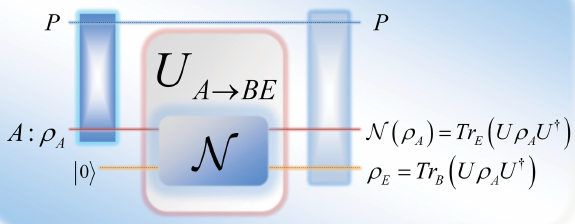
\includegraphics[width=0.6\textwidth]{figures/quantum_communication_quantum_channel.png}
    \caption{Quantum communication through a quantum channel \cite{Gyongyosi_2018}.}
\end{figure}

\subsection{Properties of Quantum Capacity}

\begin{theorem}[Non-negativity]
The quantum capacity $Q(\mathcal{N})$ of a quantum channel is non-negative.
$$Q(\mathcal{N}) \geq 0$$
\end{theorem}

\begin{proof}
Similar to the non-negativity proofs earlier, we would construct a state that achieves zero coherent information. Since the quantum capacity is the maximum over all such states, it is guaranteed to be non-negative.

Consider the input state $\phi_{AA'}$ to be a product state of the form $\psi_A \otimes \Phi_{A'}$, where the state $A$ is pure. We can evaluate its coherent information as follows.

\begin{align*}
I(A \rangle B)_{\psi \otimes \mathcal{N}(\Phi)} &= S(B)_{\mathcal{N}(\Phi)} - S(AB)_{\psi \otimes \mathcal{N}(\Phi)} \\
&= S(B)_{\mathcal{N}(\Phi)} - S(A)_{\psi} - S(B)_{\mathcal{N}(\Phi)} \\
&= - S(A)_{\psi} \\
&= 0
\end{align*}

The first equality follows from the definition of coherent information. The second makes use of the fact that $AB$ is a product state. The third cancels out common terms, while the fourth makes use of the fact that $A$ is a pure state.
\end{proof}

\begin{theorem}[Non-additivity]
Let $\mathcal{N}_1$ and $\mathcal{N}_2$ represent two quantum channels. The quantum capacity of the combined quantum channel $\mathcal{N}_1 \otimes \mathcal{N}_2$ is not equal to the sum of the individual private capacities of $\mathcal{N}_1$ and $\mathcal{N}_2$.
$$Q(\mathcal{N}_1 \otimes \mathcal{N}_2) \neq Q(\mathcal{N}_1) + Q(\mathcal{N}_2)$$
\end{theorem}

\begin{proof}
Consider a private Horodecki channel $\mathcal{N}_H$ and a symmetric channel of unbounded dimension $\mathcal{A}$. These channels are known to have the following properties \cite{Horodecki_1996} \cite{Horodecki_1997} \cite{Smith_2008_Symmetric}.
$$P(\mathcal{N}_H) > 0, Q(\mathcal{N}_H) = 0, Q(A) = 0$$

Further, we will utilize the following relation between the private capacity and the assisted capacity \cite{Smith_2008}.
$$\frac{1}{2} P(N_H) \leq Q_A(N_H)$$

Since $P(\mathcal{N}_H) > 0$, it follows that the assisted capacity $Q_A(\mathcal{N}_H) > 0$. Further, since $A$ is a symmetric channel of unbounded dimension, the quantum capacity of the joint channel can be related with the assisted capacity as follows \cite{Smith_2008_Symmetric}.
$$Q(\mathcal{N}_H \times A) = Q_A(\mathcal{N}_H) > 0$$

Finally, note that $Q(\mathcal{N}_H) + Q(A) = 0$. We can thus conclude the following relation establishing non-additivity.
$$Q(\mathcal{N}_H \times A) \neq Q(\mathcal{N}_H) + Q(A)$$
\end{proof}

\begin{theorem}[Relation with other capacities]
The single use capacities of a quantum channel $\mathcal{N}$ are related to each other as:
$$Q(\mathcal{N}) \leq P(\mathcal{N}) \leq C(\mathcal{N})$$
\end{theorem}

\begin{proof}
The reason why $P(\mathcal{N}) \leq C(\mathcal{N})$ holds is easy to see. In both classical and private communication models, our objective is to transmit classical information. Private communication is a specific case of the lesser constrained classical communication through quantum channels. Thus, the classical capacity cannot be lesser than the private capacity.

For proving the other half of the inequality, i.e. $Q(\mathcal{N}) \leq P(\mathcal{N})$, we will consider a pure state that maximizes the quantum capacity. Let $\sigma_{XA'}$ denote the augmented classical-quantum state that correlates with index $x$.
$$\sigma_{XA'} = \sum_{x} p_X(x) \ket{x}\bra{x} \otimes \ket{\phi_x}\bra{\phi_x}_{A'}$$

\begin{align*}
Q(\mathcal{N}) &= \max_{\rho} \left[ S(B)_{\rho} - S(E)_{\rho} \right] \\
&= S(B)_{\sigma} - S(E)_{\sigma}\\
&= S(B)_{\sigma} - S(B|X)_{\sigma} - S(E)_{\sigma} + S(B|X)_{\sigma}\\
&= I(X;B)_{\sigma} - I(X;E)_{\sigma} \\
&\leq \max_{\rho} \left[ I(X;B)_{\rho} - I(X;E)_{\rho} \right] \\
&\leq P(\mathcal{N})
\end{align*}
\end{proof}
